\section{Results}
\label{sec:results}
\begin{figure*}[hb]
  \centering

  \begin{subfigure}[t]{0.475\tw}\centering
    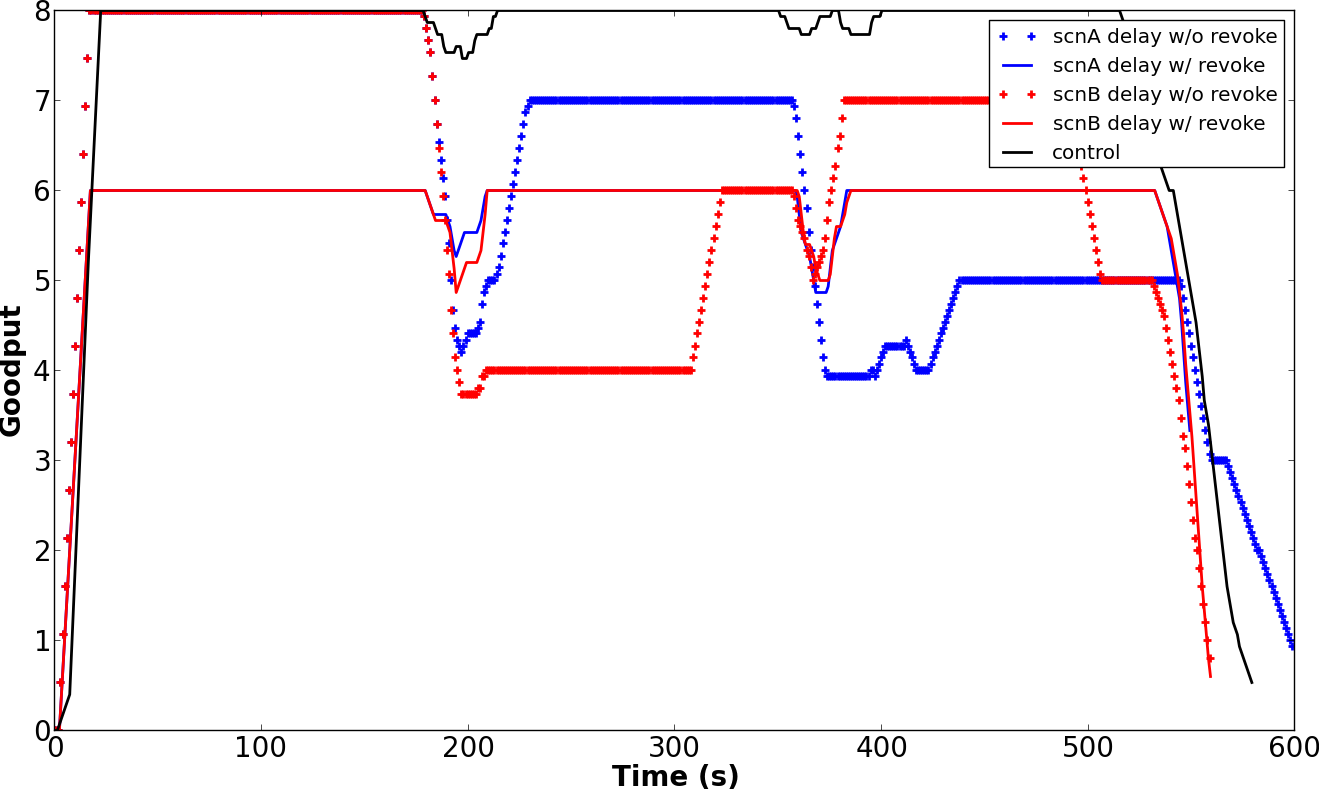
\includegraphics[width=\textwidth]{../results/control_greedy_goodput.png}
    \caption{Goodput Results for Framework 1}
    \label{fig:greedy-goodput}
  \end{subfigure}%
  \hfill
  \begin{subfigure}[t]{0.475\tw}\centering
    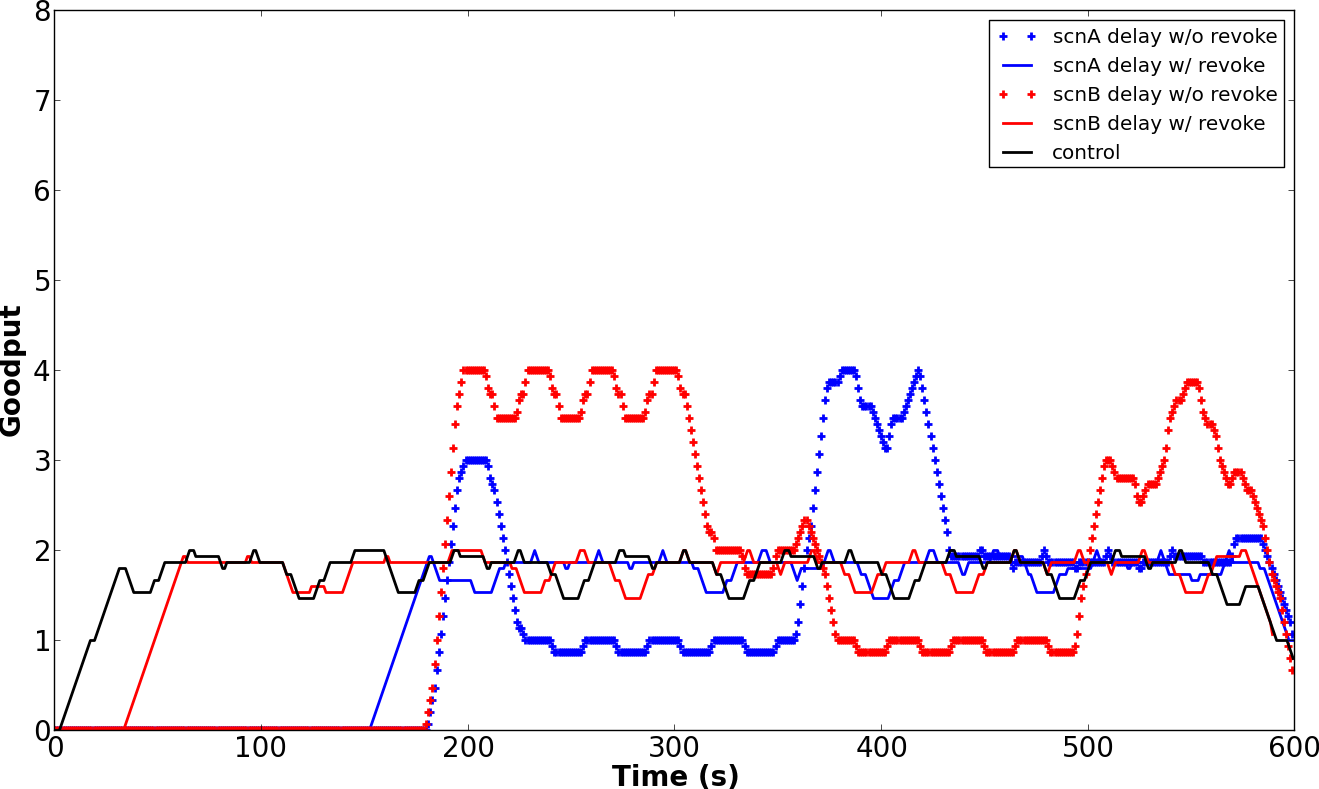
\includegraphics[width=\textwidth]{../results/control_model_goodput.png}
    \caption{Latency Results for Framework 2}
    \label{fig:model-goodput}
  \end{subfigure}%

  \caption{\textbf{Goodput Results For Frameworks 1 and 2}
  Figure~\ref{fig:greedy-goodput} and Figure~\ref{fig:model-goodput} plots the goodput results for 
  Framework 1 and Framework 2 respectively. The black lines correspond to the case where the frameworks
  are running in isolation. The blue lines correspond to Scenario A while the red lines correspond to
  Scenario B. Solid lines correspond to the case where resource revocation is used while $+$ lines
  correspond to the case when no resource revocation is used.
  }
  \label{fig:control-goodput}
\end{figure*}

\begin{figure*}[hb]
  \centering

  \begin{subfigure}[t]{0.475\tw}\centering
    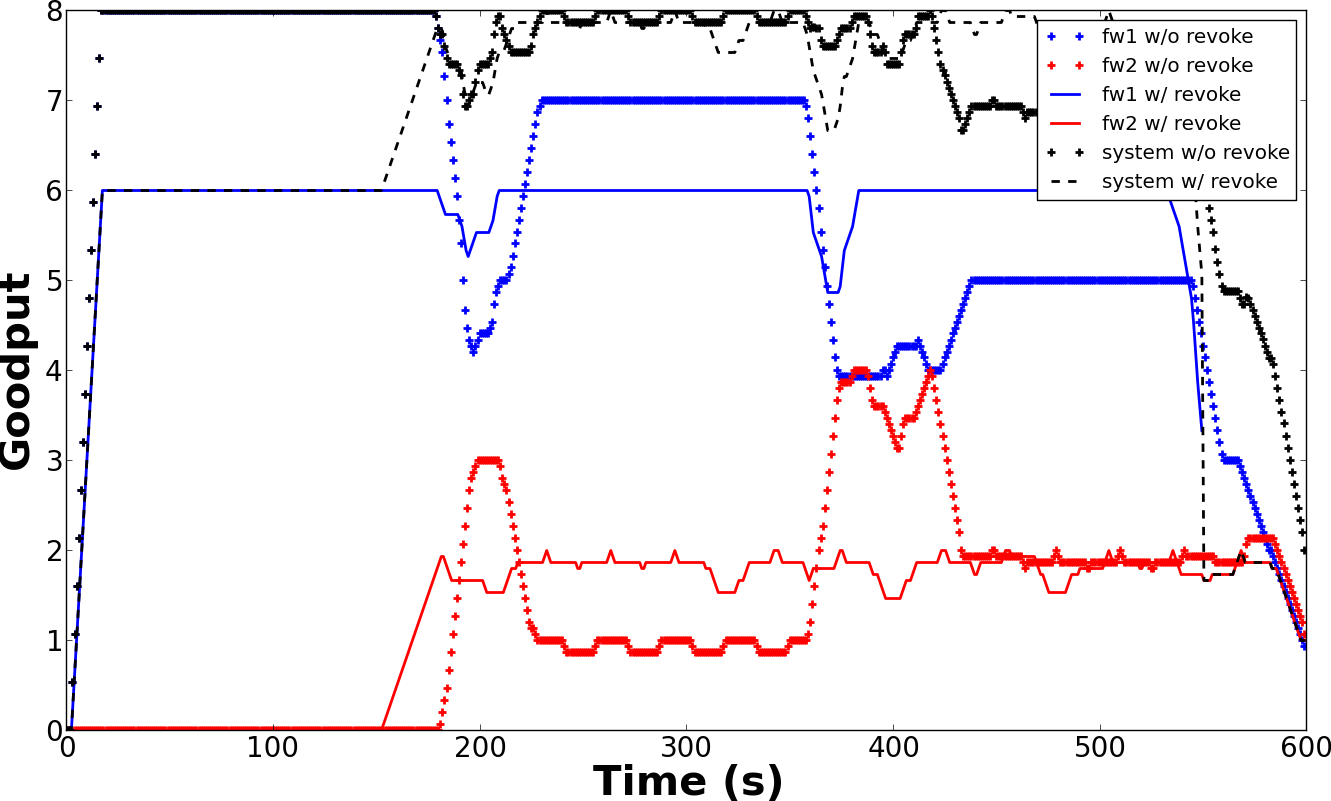
\includegraphics[width=\textwidth]{../results/150_goodput.png}
    \caption{Goodput Results for Scenario A}
    \label{fig:150-goodput}
  \end{subfigure}%
  \hfill
  \begin{subfigure}[t]{0.475\tw}\centering
    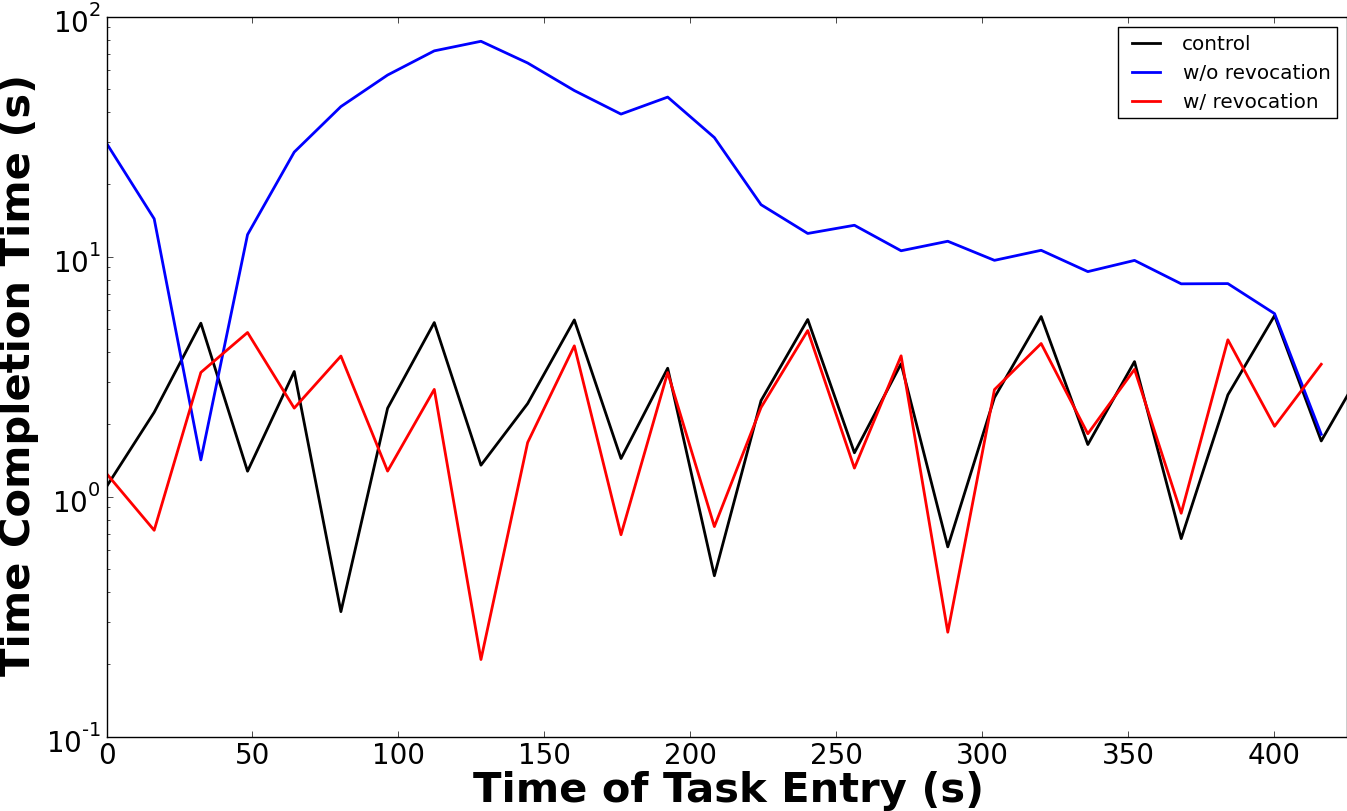
\includegraphics[width=\textwidth]{../results/150_fw_latency.png}
    \caption{Latency Results for Scenario A}
    \label{fig:150-latency}
  \end{subfigure}%

  \caption{\textbf{Goodput and Latency Results for Scenario A}
  Figure~\ref{fig:150-goodput} shows that
  there is significant goodput loss at the beginning due to the fact that tasks that have been running
  for 150 seconds are killed. However, this drastically improves the latency of the second figure as
  seen in Figure~\ref{fig:150-latency}. Without resource revocation, the second framework would have
  latency numbers an order of magnitude larger than in the control. With revocation, the second
  framework's latency numbers matches closely with the control's.}
  \label{fig:150-goodput-latency}
\end{figure*}

\begin{figure*}[hb]
  \centering

  \begin{subfigure}[t]{0.475\tw}\centering
    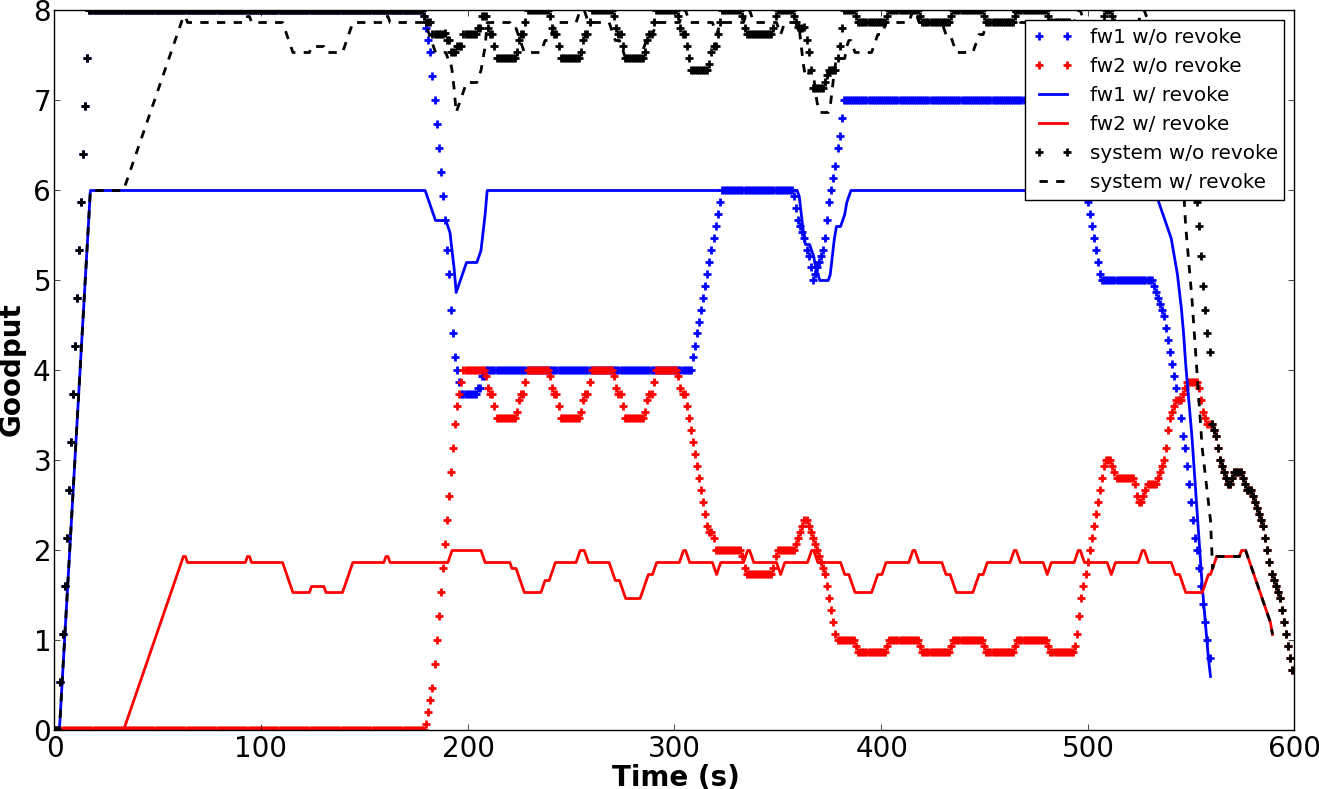
\includegraphics[width=\textwidth]{../results/30_goodput.png}
    \caption{Goodput Results for Scenario B}
    \label{fig:30-goodput}
  \end{subfigure}%
  \hfill
  \begin{subfigure}[t]{0.475\tw}\centering
    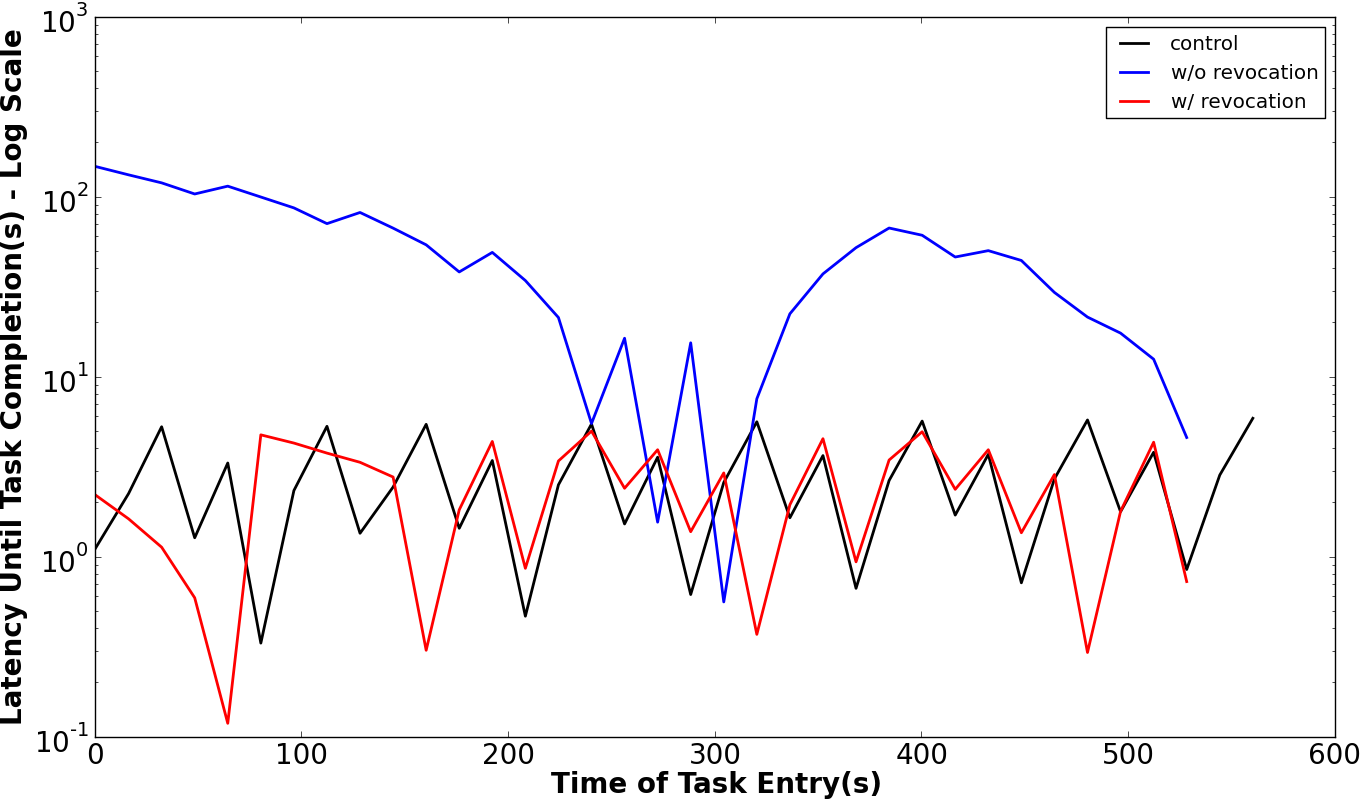
\includegraphics[width=\textwidth]{../results/30_fw_latency.png}
    \caption{Latency Results for Scenario B}
    \label{fig:30-latency}
  \end{subfigure}%

  \caption{\textbf{Goodput and Latency Results for Scenario B}
  Figure~\ref{fig:30-goodput} shows that there is still a fair amount of goodput loss in this scenario
  but the amount loss is much less than the amount in Scenario A. This is due to because the tasks
  that are killed have only made 30 seconds of progress whereas in Scenarios A the killed tasks have
  made 150 seconds of progress. Note that in this scenario, the second framework will experience
  a latency 2 orders of magnitude larger due to the fact, without resource revocation, they would have
  to wait even longer before they are given a slot in the system.
  }
  \label{fig:30-goodput-latency}
\end{figure*}

\subsection{Experimental Setup}
Unfortunately, we did not have access to a large cluster to run Mesos on. We instead ran our
experimentation on 8-core 2.67 GHz Intel Xeon processor with 49 GB of usable memory. In all of our
experiments, we used 1 instance of a Mesos Master managing 1 Slave in charge of a 8 slot ``cluster''.
Due to compute resource limitations, the experimental setup is not meant to be representative of a real
Mesos cluster. However, since we designed our synthetic frameworks to highlight specific problem 
scenarios in a Mesos cluster and not for big-picture catch-all experiments, the experimental results
are still highly beneficial.

\subsection{Offer Revocation}
Something something offer revocation.

\subsection{Resource Revocation}
For this experiment, we designed two frameworks. The first framework, Framework A, models a greedy
data analysis framework that wants as much compute resources as possible. It launches long lived tasks
that lasts 3 minutes. If allowed to run in isolation, it will easily take up a large share of the 
cluster. In our experimental setup, we allowed framework A to take up all 8 slots. Framework B, on the
other hand, models reactive realtime jobs. Every 15 seconds it generates and launches 2 short-lived 
tasks spanning 30 seconds each. If allowed to run in isolation, this framework will only use up two 
slots in the cluster. 

Before diving into our experiments, we first allow Frameworks A and B to run in the cluster isolation to
verify that they behave as intended and to have a good reference point for our experiments. The solid
black lines in Figure~\ref{fig:greedy-goodput} and Figure~\ref{fig:model-goodput} correspond to 
achievable goodput results when the frameworks are allowed to run by themselves. As expected, 
Framework A will eat up all 8 slots while Framework B will never take up more than 2 slots even if 
Mesos offers it more resources. The solid black lines in Figure~\ref{fig:150-latency} and
Figure~\ref{fig:30-latency} corresponds to the achievable latency when Framework B is allowed to run by
itself in the cluster.

We closely examined two extreme corners of operation. Figure~\ref{fig:150-goodput-latency} documents our
results for Scenario A. In this scenario, we have Framework A enter the system first. Since it is the 
only framework in the system, it quickly takes up all 8 slots in the system. We then have framework B
enter the system 150 seconds later. We first examine how our system behaves without resource revocation.
We'll then show how resource revocation improves the performance of our system. Recall that Framework's
A task each last 3 minutes. This means that without resource revocation, framework B would only have to
wait 30 seconds for Framework A's task to finish at which point Mesos can then make an offer to 
Framework B. Furthermore, since Framework B generates tasks every 15 seconds, regardless of whether or
not Mesos is able to make it a resource offer, by the time Mesos is able to make it an offer, 
framework B will have a pile up of tasks in its task queue. It will thus grab a larger share of the 
system. This behavior can be seen by the red $+$ line in Figure~\ref{fig:150-goodput}. Notice that at 
180s, this line will jump up to 3. It will then quickly drop to 1. This is because Framework B only 
requires 2 slots to keep its task queue empty and having more slots means that it will complete tasks 
faster than it can generate tasks. It will therefore relinquish two of its three slots to framework A.
This will cause the tasks in its task queue to pile up again. So then at time 360, when framework A's
second set of tasks completes, Framework B will take up four slots in the system. This behavior can
also be seen by Frmaework B's latency (the solid blue line in Figure~\ref{fig:150-latency}). Notice how
initially Framework B's tasks have latency an order of magnitude larger than the control case (the
solid black line). However, this latency will quickly drop (because Framework B has a much larger share
of the system than it needs) before spiking up again (because it has a smaller share of the system
than it needs).

Now we'll examine what happens when we allow Mesos to revoke resources. The solid blue and red lines
indicate the behaviors of Framework A and Framework B with revocation respectively. First, notice that
framework B immediately starts at time 150, when it enters the system whereas before it was not able
to start until time 180, as indicated by the red $+$ line. Furthermore, Framework B's goodput remains
steady throughout its run, fully utilizing its two slots in the system. And finally, Framework B's tasks
experiences latency that matches closely with the control case (compare the red line to the black line
in Figure~\ref{fig:150-latency}). Although resource revocation improves Framework B's performance, it 
also introduces some drawbacks into the system that were not previously there. Compare the system's 
goodput with revocation (the solid black line in Figure~\ref{fig:150-goodput}) to the system's goodput
without resource revocation (the dashed line in Figure~\ref{fig:150-goodput}). Notice that there is a
drop in goodput from time 0 to time 150. This is due to the fact that two of Framework A's tasks are 
killed at time 150. Thus any work that those two tasks made from time 0 to time 150 is lost. However,
this is the only time that the system loses goodput.
